\documentclass[a4paper]{article}

\def\nterm {April}
\def\nyear {2024}
\def\nlecturer {Ryan Tibshirani}
\def\ncourse {Convex Optimization: Fall 2019}

../header.tex

\begin{document}
\maketitle
{\small
\noindent\textbf{Course Information}\\ 
\indent \textbf{Instructor:} \textcolor{blue}{\href{https://www.stat.berkeley.edu/~ryantibs/index.html}{\nlecturer}} \\
\indent\textbf{Homepage:} \textcolor{blue}{\href{https://www.stat.cmu.edu/~ryantibs/convexopt/}{Machine Learning 10-725}} \\
\indent\textbf{Teaching:} Carnegie Mellon University \\

\vspace{10pt}
\noindent\textbf{Schedule}\\
\indent This course is divided into five parts: 
\begin{enumerate}
    \item \textbf{Theory I: Fundamentals}
    \begin{itemize}
        \item Introduction
        \item Convexity I: Sets and Functions
    \end{itemize}
    \item \textbf{Algorithms I: First-order methods}
    \item \textbf{Theory II: Duality and optimality}
    \item \textbf{Algorithms II: Second-order methods}
    \item \textbf{Advanced topics}
\end{enumerate}

\tableofcontents

% \setcounter{section}{0}
% \section{Introduction}


% \begin{defi}[Optimization problem] 
%     \begin{align*}
%         \min _{x \in D} & \quad f(x) \\
%         \text { subject to } &\quad g_{i}(x) \leq 0, \ i=1, \ldots, m \\
%         &\quad h_{j}(x)=0, \ j=1, \ldots, r
%     \end{align*}
% \end{defi}
% Here $D = \dom (f) \cap \bigcap_{i=1}^{m} \dom (g_{i}) \cap \bigcap_{j=1}^{r} \dom(h_j)$, common domain of all functions.

% \begin{figure}[htbp] 
%   \centering 
%   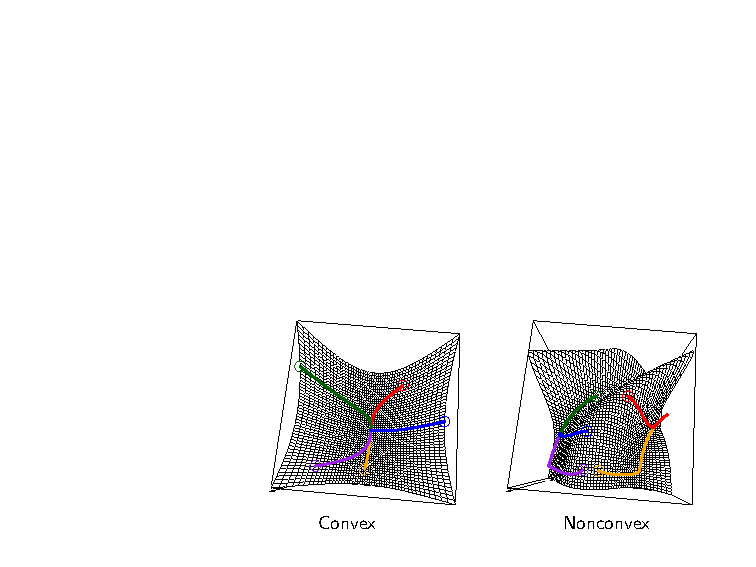
\includegraphics[width=0.6\textwidth]{img/convex_vs_nonconvex.pdf} 
% \end{figure}

% This is a \textbf{convex optimization problem} provided the functions $f$ and $g_i, i=1,\ldots,m$ are convex, and  $h_j, j=1,\ldots,r$ are affine:
% \[
%     h_j (x) = a_{j}^{T}x + b_j, \quad j =1,\ldots,r
% \]

% For convex optimization problem, \textbf{local minima are global minima}.
% Formally, if $x$ is feasible---$x \in D$, and satisfies all constraints and minimizes $f$ in a local neighborhood,
% \[
%     f(x) \leq f(y) \text{\ for \ all \ feasible} \ y, \ \left\lVert x -y \right\rVert_2 \leq \rho
% \]
% then
% \[
%     f(x) \leq f(y) \text{\ for \ all \ feasible} \ y
% \]

\section{Convexity I: Sets and Functions}
\subsection{Convex sets}
\begin{defi}[Convex set]
  $C \subseteq \R^n$ such that 
  \[
      x, y \in C \Longrightarrow  tx + (1-t)y \in C,\text{\ for\ all}\ 0 \leq t \leq 1 
  \]
\end{defi}

\begin{figure}[htbp] 
  \centering 
  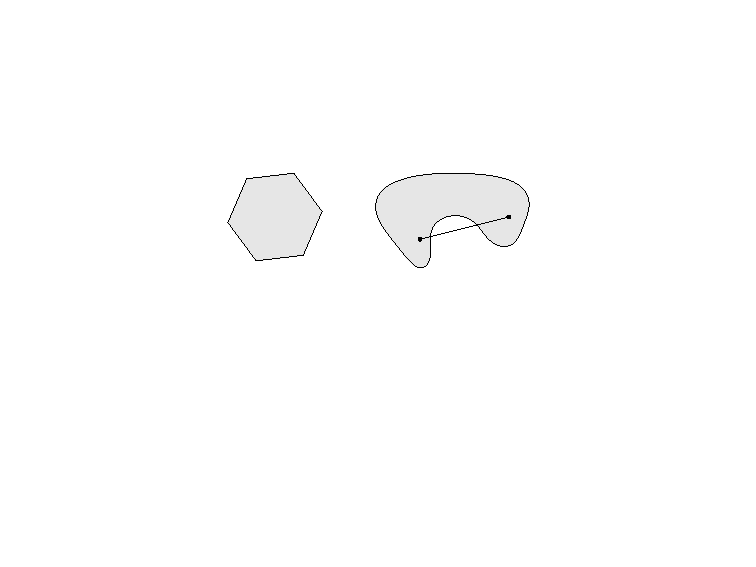
\includegraphics[width=0.6\textwidth]{img/convex_set.pdf} 
\end{figure}

\begin{defi}[Convex combination] 
  For $x_1,\cdots,x_k \in \mathbb{R}^n$, any linear combination
  \[
    \theta_1 x_1 + \cdots + \theta_k x_k
    \]
  with $\theta_i \geq 0, i=1,\cdots, k$, and $\sum_{i = 1}^{k}\theta_i = 1$. 
\end{defi}

\begin{defi}[Convex hull] 
  The convex hull of $ C $, conv($C$), is all convex combinations of elements, and is always convex.
\end{defi}

\subsubsection{Example of convex sets:}
\begin{enumerate}
  \item \textbf{Trivial ones:} empty set, point, line 
  \item \textbf{Norm ball:} $\{x: \Vert x \Vert \leq r \}$, for given norm $\Vert \cdot \Vert$, radius $r$
  \item \textbf{Hyperplane:} $\{x: a^T x = b \}$, for given $a, b$
  \item \textbf{Halfspace:} $\{x: a^T x \leq b \}$, for given $a, b$
  \item \textbf{Affine space:} $\{x: A x = b \}$, for given $A, b$
  \item \textbf{Polyhedron:} $\{x: A x \leq b \}$, while inequality $\leq$ is interpreted componentwise. Note: the set $\{x: A x \leq b, Cx = d \}$ is also a Polyhedron
  \item \textbf{Simplex:} special case of polyhedra, given by conc$\{x_0,\cdots,x_k \}$, where these points are affinely independent. The canonical example is the \textbf{probability simplex},
  \[
    \text{conv}\{ e_1,\cdots,e_n\} = \{w: w \geq 0, 1^T w = 1\}
    \]
\end{enumerate}

\subsubsection{Key properties of convex sets:}
\begin{enumerate}
  \item \textbf{Separating hyperplane theorem:} two disjoint convex sets have a separating between hyperplane them
  Formally, if $C, D$ are nonempty convex sets with $C\cap  D = \emptyset $, then there exists $a, b$ such that
  \begin{align*}
    C & \subseteq \{x : a^T x \leq b\} \\
    D & \subseteq \{x : a^T x \geq b\} 
  \end{align*}
  \item \textbf{Supporting hyperplane theorem:} a boundary point of a convex set has a supporting hyperplane passing through it. Formally, if $C$ is a nonempty convex set, and $x_0 \in \text{bd}(C)$, then there exists $a$ such that 
  \begin{equation}
    C \subseteq \{x : a^T x \leq a^T x_0\} 
  \end{equation}
\end{enumerate}

\begin{figure}[htbp] 
  \centering 
  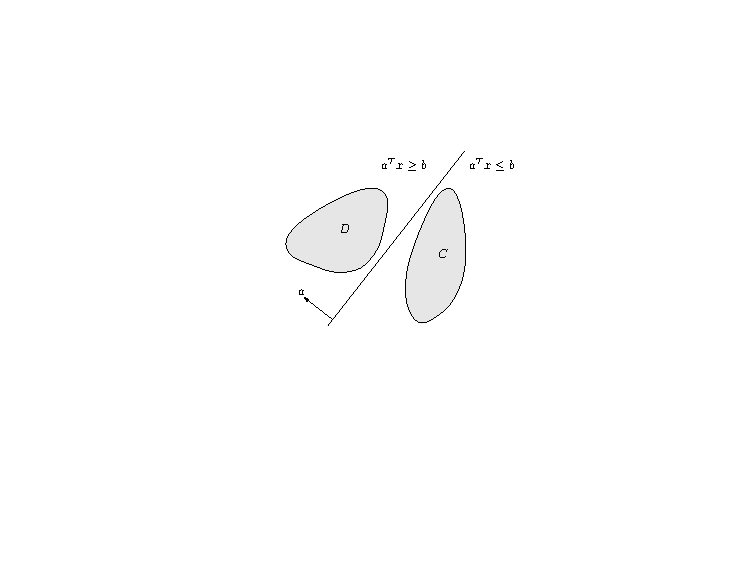
\includegraphics[width=0.4\textwidth]{img/hyperplane_separating.pdf} 
\end{figure}

\subsubsection{Operations preserving convexity}
\begin{enumerate}
  \item \textbf{Intersection:} the intersection of convex sets is convex
  \item \textbf{Scaling and translation:} if $C$ is convex, then
  \[ 
    aC + b = \{ax+ b : x \in C\}
    \]
  is convex for any $a, b$
  \item \textbf{Affine images and preimages:} if $f(x) = Ax +b$ and $C$ is convex then 
  \begin{equation}
    f(C) = \{f(x) : x \in C\}
  \end{equation}
  is convex, and if $D$ is convex then 
  \begin{equation}
    f^{-1}(D) = \{x: f(x) \in D\}
  \end{equation}
  is convex
  \item \textbf{Perspective images and preimages:} the perspective function is $P : \mathbb{R}^n \times \mathbb{R}_{++} \rightarrow \mathbb{R}^n$ where $ \mathbb{R}_{++}$ denotes positive reals,
  \[ 
    P(x, z) = x / z
    \]
  for $ z > 0$. If $C \subseteq \text{dom}(P)$ is convex then so is $P(C)$, and if $D $ is convex then so is $P^{-1}(D)$
  \item  \textbf{Linear-fractional images and preimages:} the perspective map composed with an affine function,
  \[ 
    f(x) = \frac{Ax + b}{c^T x + d}
    \]
  is called a linear-fractional function, defined on $c^T x + d > 0$. If $C \subseteq \text{dom}(f)$ is convex then so if $f(C)$, and if $D$ is convex then so is $f^{-1}(D)$ 
\end{enumerate}

\subsection{Cones}
\begin{defi}[Cone]
  $C \subseteq \mathbb{R}^n$ such that  
  \[
    x \in C \Longrightarrow  tx \in C,\text{\ for\ all}\ t \geq 0 
  \]
\end{defi}

\begin{defi}[Convex cone]
  Cone that is also convex, i.e.,
  \[
    x_1, x_2 \in C \Longrightarrow  t_1 x_1 + t_2 x_2 \in C,\text{\ for\ all}\ t_1, t_2 \geq 0 
  \]
\end{defi}

\begin{defi}[Conic combination]
  For $x_1,\cdots,x_k \in \mathbb{R}^n$, any linear combination
  \[
    \theta_1 x_1 + \cdots + \theta_k x_k
    \]
  with $\theta_i \geq 0, i=1,\cdots, k$.
\end{defi}

\begin{defi}[Conic hull]
  The conic hull of $ C $, cone($C$), is all conic combinations of elements.
\end{defi}

\subsubsection{Example of convex cones:}
\begin{enumerate}
  \item \textbf{Norm cone:} $\{(x,t) : \Vert x \Vert \leq r \}$, for a norm $\Vert \cdot \Vert$. Under the $\ell_2$ norm $\Vert \cdot \Vert_2$, called second-order cone
  \item \textbf{Normal cone:} given any set $C$ and point $x \in C$, we can define
  \[
    \mathcal{N}_C (x) = \{g : g^T x \geq g^T y, \text{\ for \ all} \ y \in C\} 
    \]
  This is always a convex cone, regardless of $C$
  \item \textbf{Positive semidefinite cone:} $\mathbb{S}^n_+ = \{X \in \mathbb{S}^n : X \succeq 0 \}$, where $X \succeq 0 $ means that $X$ is positive semidefinite (and $\mathbb{S}^n$ is the set of $n \times n$ symmetric matrices)
\end{enumerate}

\subsection{Convex function}
\begin{defi}[Convex function]
  $f: \R^n \rightarrow \R$ such that $\dom (f) \subseteq \R^n$ convex, and 
  \[
      f(tx + (1-t)y) \leq tf(x) + (1-t)f(y),\text{\ for\ all}\ 0 \leq t \leq 1 
  \]
  and all $x, y \in \dom (f)$
\end{defi}

\begin{center}
\begin{tikzpicture}
  \draw (0.27, 0.5) -- (3, 1);
  \draw (0, 1) .. controls (1,-1) .. (3.5, 1.5);
  \node  at (0.27, 0.5) [circ] {}; 
  \node at (0.27, 0.5) [left] {$(x, f(x))$};
  \node at (3, 1) [circ] {};
  \node at (3, 1) [right] {$(y, f(y))$};
\end{tikzpicture}
\end{center}

\begin{defi}[Concave function] 
$f: \R^n \rightarrow \R$ such that $\dom (f) \subseteq \R^n$ convex, and 
\[
    f(tx + (1-t)y) \geq tf(x) + (1-t)f(y),\text{\ for\ all}\ 0 \leq t \leq 1 
\]
and all $x, y \in \dom (f)$, so that 
\[
  f \ \text{concave} \Leftrightarrow -f \ \text{convex}
\]
\end{defi}

\noindent \textbf{Important modifiers:}
\begin{enumerate}
\item \textbf{Strictly convex:} $f(tx + (1-t)y) < tf(x) + (1-t)f(y),\text{\ for} \ x \neq y $ and $ 0 < t < 1$. In words, $f$ is convex and has greater curvature than a linear function
\item \textbf{Strongly convex:} with parameter  $m > 0: f - \frac{m}{2} \Vert x \Vert_2^2$ is convex. In words, $f$ is at least as convex as a quadratic function
\item \textbf{Note:} strongly convex $\Rightarrow $ strictly convex $\Rightarrow$ convex (Analogously for concave functions)
\end{enumerate}

\subsubsection{Example of convex functions}
\begin{enumerate}
  \item \textbf{Univariate functions:}
  \begin{enumerate}
    \item Exponential function: $e^{ax}$ is convex for any $a$ over $\mathbb{R}$
    \item Power function: $x^a$ is convex for $a \geq 1$ or $a \leq 0$ over $\mathbb{R}_+$ (nonnegative reals)
    \item Power function: $x^a$ is concave for $0 \leq a \leq 1$ over $\mathbb{R}_+$
    \item Logarithmic function: $\log (x)$ is concave over $\mathbb{R}_{++}$  
  \end{enumerate}
  \item \textbf{Affine function:} $a^T x + b$ is both convex and concave
  \item \textbf{Quadratic function:} $\frac{1}{2} x^T Q x + b^T x + c$ is convex provided that $Q \succeq 0$ (positive semidefinite)
  \item \textbf{Least squares loss:} $\Vert y - Ax \Vert^2_2$ is always convex (since $A^T A$ is always positive semidefinite) 
  \item \textbf{Norm:} $\Vert x \Vert$ is convex for any norm; e.g. $\ell_p$ norms,
  \[
    \Vert x \Vert_p = (\sum_{i=1}^n |x_i|^p)^{1/p} \ \text{for} \ p \geq 1, \quad \Vert x \Vert_\infty = \max\limits_{i=1,\cdots.n}|x_i|
  \]
  and also operator (spectral) and trace (nuclear) norms,
  \[
    \Vert X \Vert_{op} = \sigma_1(X), \Vert X \Vert_{tr} = \sum_{i=1}^r \sigma_r(X)
  \]
  where $\sigma_1(X) \geq \cdots \geq \sigma_r(X) \geq 0$ are the singular values of the matrix $X$
  \item \textbf{Indicator function:} if $C$ is convex, then its indicator function
  \[
    I_C(x) = 
    \begin{cases}
      0 &\ x \in C \\
      \infty &\ x \notin C
    \end{cases}
  \]
  \item \textbf{Support function:} for any set $C$(convex or not), its indicator function 
  \[
    I_C^*(x) = \max\limits_{y \in C} x^T y  
  \]
  is convex 
  \item \textbf{Max function:} $f(x) = \max \{ x_1, \cdots, x_n \}$ is convex 

\end{enumerate}

\subsubsection{Key properties of convex functions}
\begin{enumerate}
  \item A function is convex if and only if its restriction to any line is convex
  \item \textbf{Epigraph characterization:} a function $f$ is convex if and only if its epigraph
  \[
    \text{epi}(f) = \{(x,t) \in \text{dom}(f) \times \mathbb{R} : f(x) \leq t \}
  \]
  is a convex set
  \item \textbf{Convex sublevel sets:} if $f$ is convex, then its sublevel sets 
  \[
    \{x \in \text{dom}(f) : f(x) \leq t \}
  \]
  are convex, for all $t \in \mathbb{R}$. The converse is not true
  \item \textbf{First order characterization:} if $f$ is differentiable, then $f$ is convex if and only if dom($f$) is convex, and
  \[
    f(y) \geq f(x) + \nabla f(x)^T(y-x)
  \]
  for all $x, y \in $ dom($f$). Therefore for a differentiable convex function $ \nabla f(x) = 0 \Leftrightarrow x$ minimizes $f$
  \item \textbf{Second order characterization:} if $f$ is twice differentiable, then $f$ is convex if and only if dom($f$) is convex, and $\nabla^2 f(x) \succeq 0$ for all $x \in $ dom($f$)
  \item \textbf{Jensen's inequality:} if $f$ is convex, and $X$ is a random variable supported on dom($f$), then $f(\mathbb{E}[X]) \leq \mathbb{E}[f(x)]$
\end{enumerate}

\subsubsection{Operations preserving convexity}
\begin{enumerate}
  \item \textbf{Nonnegative linear combination:} $f_1,\cdots,f_m$ convex implies $a_1f_1 + \cdots + a_mf_m$ convex for any $a_1,\cdots,a_m \geq 0$
  \item \textbf{Pointwise maximization:} if $f_s$ is convex for any $s \in S$,then $f(x) = \max_{s \in S} f_s(x)$ is convex. Note that the set $S$ here (number of functions $f_s$) can be infinite
  \item \textbf{Partial minimization:} if $g(x,y)$ is convex in $x, y$, and $C$ is convex, then $f(x) = \min_{y \in C}g(x,y)$ is convex
  \item \textbf{Affine composition:} if $f$ is convex, then $g(x)=f(Ax+b)$ is convex
  \item \textbf{General composition:} suppose $f = h\circ g$, where $g : \mathbb{R}^n \rightarrow \mathbb{R}$, $h : \mathbb{R} \rightarrow \mathbb{R}$, $f : \mathbb{R}^n \rightarrow \mathbb{R}$. Then:
  \subitem $f$ is convex if $h$ is convex and nondecreasing, $g$ is convex
  \subitem $f$ is convex if $h$ is convex and nonincreasing, $g$ is concave
  \subitem $f$ is concave if $h$ is concave and nondecreasing, $g$ is concave
  \subitem $f$ is concave if $h$ is concave and nonincreasing, $g$ is convex
  \item \textbf{Vector composition:} suppose that
  \[
    f(x) = h(g(x)) = h(g_1(x), \cdots, g_k(x))
  \]
  where $g : \mathbb{R}^n \rightarrow \mathbb{R}^k$, $h : \mathbb{R}^k \rightarrow \mathbb{R}$, $f : \mathbb{R}^n \rightarrow \mathbb{R}$. Then:
  \subitem $f$ is convex if $h$ is convex and nondecreasing in each argument, $g$ is convex
  \subitem $f$ is convex if $h$ is convex and nonincreasing in each argument, $g$ is concave
  \subitem $f$ is concave if $h$ is concave and nondecreasing in each argument, $g$ is concave
  \subitem $f$ is concave if $h$ is concave and nonincreasing in each argument, $g$ is convex
\end{enumerate}


\end{document}